\section{\algname{}: Context-to-Harness Skill Compilation}
\label{sec:method}

We present \algname{}, a framework for online harness learning. The goal is to convert one-shot execution contexts into a reusable harness that guides future task solving. Unlike experience retrieval, which recalls past cases, \algname{} compiles noisy execution signals into structured guidance that can shape later planning, acting, verification, and recovery.

Figure~\ref{fig:main} gives an overview. \algname{} maintains a current harness that guides the solver before execution, shaping how it plans, acts, verifies, and recovers. After each task batch, execution contexts are reflected into candidate memories and compiled back into the harness as cross-task patterns and task-type procedures, allowing the updated harness to guide later executions.
\begin{figure*}[t]
    \centering
    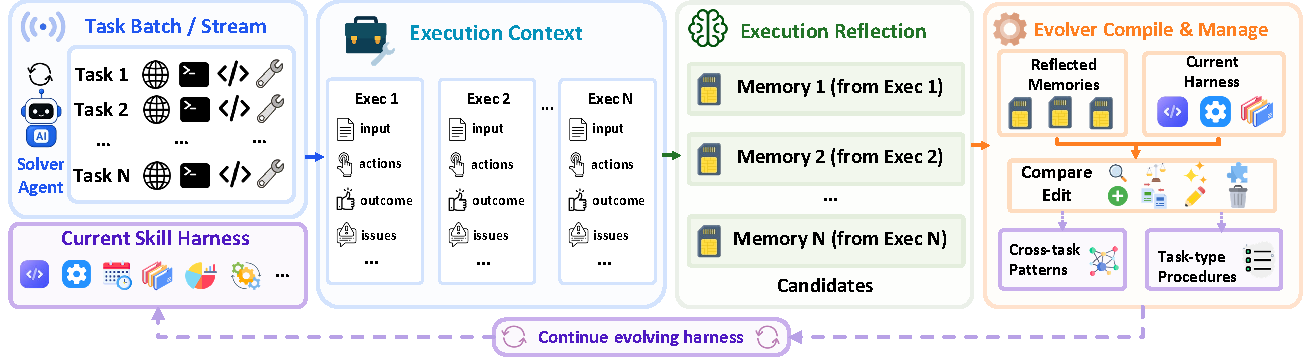
\includegraphics[width=1.03\textwidth]{figures/main.pdf}
    \caption{
    Overview of \algname{}. The solver uses the current harness to solve a task batch or stream. Each execution produces a context, including input, action trajectory, outcome, and feedback. Execution reflection converts these contexts into candidate memories. The evolver compares the candidate memories with the current harness and updates the harness with cross-task patterns and task-type procedures for later batches.
    }
    \label{fig:main}
    \vspace{-0.4cm}
\end{figure*}

\subsection{Online Harness Learning Setup}
\label{sec:method-setup}

Let $\{B_1,\ldots,B_K\}$ denote a stream of task batches, where $B_i=\{x_{i,1},\ldots,x_{i,m_i}\}$. Before batch $B_i$, the agent has a current harness $\mathcal{H}_i$, a structured set of reusable guidance entries:
\begin{equation}
    \mathcal{H}_i = \{h_i^1,\ldots,h_i^{n_i}\}.
\end{equation}
The harness is external to the frozen solver and serves as a control scaffold for later executions. Unlike raw trajectory storage, it maintains compact guidance distilled from prior executions and affects future behavior through selection and injection into the solver context.

For each task $x_{i,j}$, the agent selects a compact set of harness entries:
\begin{equation}
    \mathcal{S}_{i,j}
    =
    \mathrm{Select}(x_{i,j}, \mathcal{H}_i; b),
    \qquad
    |\mathcal{S}_{i,j}| \leq b,
\end{equation}
where $b$ is the injection budget. The selected guidance is injected into the task:
\begin{equation}
    \tilde{x}_{i,j}
    =
    \mathrm{Inject}(x_{i,j}, \mathcal{S}_{i,j}).
\end{equation}
A frozen solver $\mathcal{A}$ executes the task:
\begin{equation}
    (\tau_{i,j}, y_{i,j}, f_{i,j})
    =
    \mathcal{A}(\tilde{x}_{i,j}),
\end{equation}
where $\tau_{i,j}$ is the action trajectory, $y_{i,j}$ is the outcome, and $f_{i,j}$ is available feedback, such as verifier results, unit-test outputs, tool diagnostics, or judge feedback. The execution context is:
\begin{equation}
    c_{i,j}
    =
    (x_{i,j}, \tau_{i,j}, y_{i,j}, f_{i,j}).
\end{equation}
Online harness learning updates $\mathcal{H}_i$ into $\mathcal{H}_{i+1}$ from these execution contexts, while keeping the solver parameters fixed.

\subsection{Context-to-Harness Compilation}
\label{sec:method-compilation}

\algname{} uses two complementary stages: \emph{execution reflection} and \emph{harness evolution}. Reflection extracts learning signals from each execution. Evolution integrates those signals into the harness.

% \paragraph{Execution reflection.}
% For each execution context $c_{i,j}$, the solver produces a candidate memory:
% \begin{equation}
%     r_{i,j}
%     =
%     \mathrm{Reflect}(c_{i,j}).
% \end{equation}
% Each candidate memory is represented as:
% \begin{equation}
%     r
%     =
%     (\mathrm{lesson}, \mathrm{trigger}, \mathrm{evidence}, \mathrm{scope\_hint}).
% \end{equation}
% Reflection uses the full task-side context available immediately after execution, including the instruction, trajectory, observations, tool outputs, outcome, and feedback. This enables timely reflection over concrete failures, successful steps, and diagnostic signals before they are abstracted or lost. It does not compare against the current harness, so its output is not a final harness update, but a candidate signal extracted from the completed execution.

\paragraph{Execution reflection.}
For each completed execution context $c_{i,j}$, the solver produces a candidate memory only when the execution fails or receives negative feedback:
\begin{equation}
    r_{i,j}
    =
    \mathrm{Reflect}(c_{i,j}).
\end{equation}
Each candidate memory is represented as:
\begin{equation}
    r
    =
    (\mathrm{lesson}, \mathrm{trigger}, \mathrm{evidence}, \mathrm{scope\_hint}).
\end{equation}
Reflection uses the full task-side context available immediately after execution, including the instruction, trajectory, observations, tool outputs, outcome, and feedback. We focus reflection on failures because they expose the solver's current boundary: incorrect assumptions, missing constraints, ineffective tool use, weak verification, and failed recovery. This makes the resulting candidate memories more targeted for harness improvement, while avoiding unnecessary updates from successful executions that may contain task-specific details. The reflection stage does not compare against the current harness, so its output is not a final harness update, but a failure-grounded candidate signal extracted from the completed execution.

\paragraph{Harness evolution.}
After batch $B_i$, the candidate memories form:
\begin{equation}
    \mathcal{R}_i
    =
    \{r_{i,j}\}_{j=1}^{m_i}.
\end{equation}
The evolver receives the candidate memories and the current harness:
\begin{equation}
    \mathcal{O}_i
    =
    \mathrm{Evolver}(\mathcal{H}_i, \mathcal{R}_i),
\end{equation}
where $\mathcal{O}_i$ is a set of harness edits. Conceptually, the evolver applies:
\begin{equation}
    o
    =
    \pi_{\mathrm{evolve}}(r, \mathcal{H}_i, \mathcal{R}_i),
\end{equation}
where $o \in \{\textsc{Add}, \textsc{Merge}, \textsc{Revise}, \textsc{Skip}\}$. The evolver filters noisy or redundant memories, merges compatible signals, revises existing guidance, and promotes reusable lessons when appropriate. The updated harness is:
\begin{equation}
    \mathcal{H}_{i+1}
    =
    \mathrm{ApplyEdits}(\mathcal{H}_i, \mathcal{O}_i).
\end{equation}
This makes the harness more than a memory store: candidate memories are not appended directly, but compiled into guidance that can affect future behavior.

\subsection{Harness Levels}
\label{sec:method-skill-levels}

The evolved harness contains two levels of reusable guidance. \emph{Cross-task patterns} are compiled by comparing memories across tasks and identifying shared operational structure. \emph{Task-type procedures} preserve more localized guidance for recurring task formats, interfaces, or domains. These levels are not predefined labels for individual executions. They emerge from how the evolver filters, compares, and integrates candidate memories into the harness.

\subsection{Algorithm and Modularity}
\label{sec:method-algorithm}

Algorithm~\ref{alg:context-to-harness} summarizes \algname{}. We use batch-level updates so the evolver can both compile localized task-type procedures and compare memories across tasks to extract cross-task patterns. The same formulation reduces to task-type updating when $|B_i|=1$.

\begin{algorithm}[t]
\caption{\algname{}: Context-to-Harness Skill Compilation}
\label{alg:context-to-harness}
\begin{algorithmic}[1]
\small
\STATE \textbf{Input:} task batches $\{B_1,\ldots,B_K\}$, frozen solver $\mathcal{A}$, initial harness $\mathcal{H}_1$
\FOR{$i=1,\ldots,K$}
    \STATE $\mathcal{R}_i \gets \emptyset$
    \FOR{each task $x_{i,j}\in B_i$}
        \STATE $\mathcal{S}_{i,j}\gets \mathrm{Select}(x_{i,j},\mathcal{H}_i;b)$
        \STATE $\tilde{x}_{i,j}\gets \mathrm{Inject}(x_{i,j},\mathcal{S}_{i,j})$
        \STATE $(\tau_{i,j},y_{i,j},f_{i,j})\gets \mathcal{A}(\tilde{x}_{i,j})$
        \STATE $c_{i,j}\gets (x_{i,j},\tau_{i,j},y_{i,j},f_{i,j})$
        \STATE $r_{i,j}\gets \mathrm{Reflect}(c_{i,j})$
        \STATE $\mathcal{R}_i\gets \mathcal{R}_i\cup\{r_{i,j}\}$
    \ENDFOR
    \STATE $\mathcal{O}_i^{\mathrm{type}}\gets \mathrm{CompileTaskType}(\mathcal{H}_i,\mathcal{R}_i)$
    \STATE $\mathcal{O}_i^{\mathrm{cross}}\gets \mathrm{CompileCrossTask}(\mathcal{H}_i,\mathcal{R}_i)$
    \STATE $\mathcal{O}_i\gets \mathcal{O}_i^{\mathrm{type}}\cup \mathcal{O}_i^{\mathrm{cross}}$
    \STATE $\mathcal{H}_{i+1}\gets \mathrm{ApplyEdits}(\mathcal{H}_i,\mathcal{O}_i)$
\ENDFOR
\STATE \textbf{Output:} evolved harness $\mathcal{H}_{K+1}$ and task results
\end{algorithmic}
\end{algorithm}

Here, $\mathrm{CompileTaskType}$ preserves localized procedures, while $\mathrm{CompileCrossTask}$ extracts shared patterns across executions. The modular design is intentional: by decoupling the solver, evolver, feedback source, and initial harness state, \algname{} provides a controlled framework for systematically studying what drives online harness improvement.